

\documentclass[../../e3_tp2_main.tex]{subfiles}

\begin{document}
\chapter{}

A la hora de implementar tablas de verdad como circuitos l\'ogicos, se debe establecer un compromiso entre las siguientes caracter\'isticas del dise\~no:

\begin{itemize}
	\item Menor costo: utilizar la menor cantidad de compuertas l\'ogicas posible.
	\item Menor riesgo: tener la menor probabilidad de \textit{glitches} posible.
\end{itemize}

En este contexto, se dice que se produce un \textit{glitch} cuando la salida toma moment\'aneamente un valor que no se corresponde con lo establecido por la tabla de verdad del circuito, debido a los distintos tiempos de propagaci\'on de las compuertas utlizadas. Estos \textit{glitches} pueden ser tanto est\'aticos como din\'amicos. Esto quiere decir que pueden presentarse cuando la salida deber\'ia permanecer en el mismo estado a pesar de una variaci\'on en las entradas, para el caso est\'atico, o pueden producirse varias transiciones de un estado al otro cuando deber\'ia producirse una sola, para el caso din\'amico.

\begin{figure}[H]
	\centering
	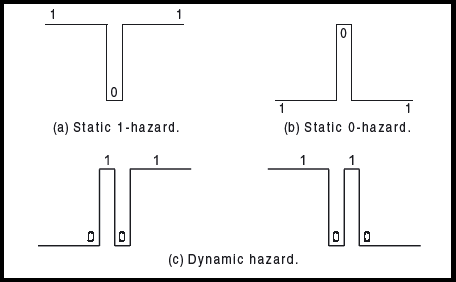
\includegraphics[scale=0.5]{hazard.png}
	\caption{\textit{Glitches} est\'aticos y din\'amicos \protect\footnotemark}
\end{figure}

\footnotetext{Imagen extra\'ida de: \url{http://www.electronicsengineering.nbcafe.in/hazards-in-digital-circuit/} (13/10/18)}
\end{document}
